\subsubsection{Experiment 2}
\begin{figure}[htbp]
	\centering
    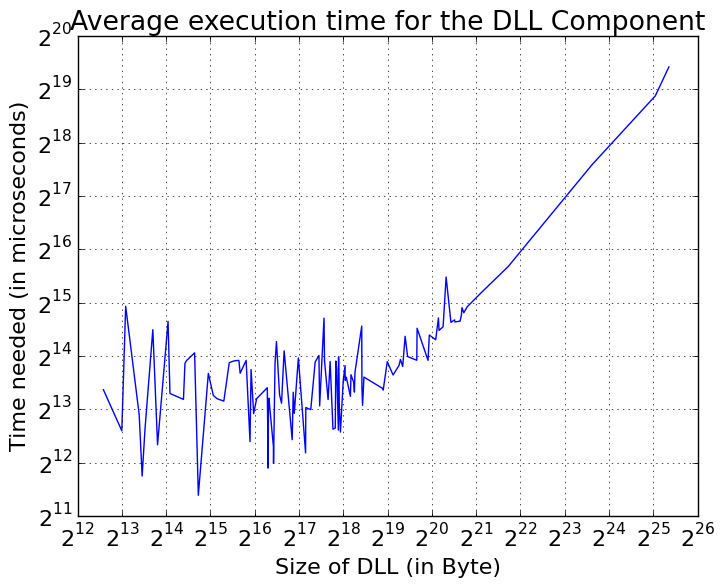
\includegraphics[width=\textwidth,height=0.45\textheight,keepaspectratio]{Evaluation/experiment2/result.png}
    \caption{Average count, 1 minute of data}
    \label{fig:ex2_result}
\end{figure}
In Experiment 2 the performance impact of the \emph{\gls{DLL}} component is evaluated. Experiment 2 uses the same hardware and software setup as Experiment 1. As the result of Experiment 1 showed, that running the \emph{\gls{DLL}} component slowed down the execution, Experiment 2 tries to find the actual reason for that result. Looking at the code, and running time measurements on it leads to the sha256 file hashing slowing down the execution. Figure \ref{fig:ex2_result} shows the result of this measurement. For file sizes between four kilobyte ($2^{12}$ byte) and one megabyte ($2^{20}$ byte), the needed time is roughly constant around 16 milliseconds ($2^{14}$ microseconds). Increasing the file size further than one megabyte results into increasing needed time for hashing the file. The graph uses logarithmic scaling with base two one both axis, which gives a better readability to the actual result. Doubling the file size starting from one megabyte will double the necessary time to create the sha256 hash.